\documentclass[tikz]{standalone}%

\usepackage[utf8]{inputenx}%  http://ctan.org/pkg/inputenx
% Euler for math | Palatino for rm | Helvetica for ss | Courier for tt
\renewcommand{\rmdefault}{ppl}% rm
\linespread{1.05}% Palatino needs more leading
\usepackage[scaled]{helvet}% ss //  http://ctan.org/pkg/helvet
\usepackage{courier}% tt // http://ctan.org/pkg/courier
\usepackage{eulervm}  %  http://ctan.org/pkg/eulervm
% a better implementation of the euler package (not in gwTeX)
\normalfont%
\usepackage[T1]{fontenc}%  http://ctan.org/pkg/fontenc
\usepackage{textcomp}%  http://ctan.org/pkg/textcomp

\usetikzlibrary{patterns}
\usetikzlibrary{intersections}
\usetikzlibrary{angles}
\usetikzlibrary{quotes}

\begin{document}
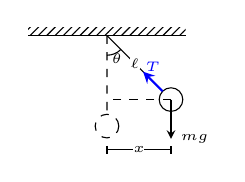
\begin{tikzpicture}
  \fill[pattern = north east lines] (-1cm, 0) rectangle (1cm, 0.1cm);

  \draw (-1cm, 0) -- (1cm, 0);
  \draw[dashed, name path = vline] (0, 0) coordinate (O) -- (0, -1cm)
  coordinate (A) (0, -1.15cm) circle[radius = 0.15cm];
  \draw (O) -- (-45:1cm) (-45:1.15cm) coordinate (B) circle[radius = 0.15cm];

  \node[font = \tiny, fill = white, inner sep = 0.01cm] at (-45:0.5cm)
  {$\ell$};
  
  \path[name path = hline] (B) -- +(-1cm, 0);
  \path[name intersections = {of = hline and vline, by = C}];

  \draw[dashed] (B) -- (C);
  \draw[thick, blue, -stealth] (-45:1cm) -- (-45:0.65cm) node[font = \tiny,
  pos = 0.5, above] {$T$};

  \path (A) -- (O) -- (B) pic["$\theta$", draw, angle radius = 0.25cm,
  angle eccentricity = 1.3, font = \tiny] {angle = A--O--B};

  \draw (0, -1.4cm) -- (0, -1.5cm);

  \path[name path = vline2] (B) -- +(0, -0.68cm);
  \path[name path = hline2] (0, -1.45cm) -- +(1cm, 0);
  \path[name intersections = {of = hline2 and vline2, by = D}];

  \draw (0, -1.45cm) -- (D) node[pos = 0.5, font = \tiny, fill = white,
  inner sep = 0.01] {$x$};
  \draw (D) -- +(0, 0.05cm);
  \draw (D) -- +(0, -0.05cm);
  \draw[-stealth] (B) -- +(0, -0.5cm) node[right, font = \tiny] {$mg$};
\end{tikzpicture}
\end{document}
%%% Local Variables:
%%% mode: latex
%%% TeX-master: t
%%% End:
